\section{Analisi dei risultati}
\label{cap:performance-analysis}

\subsection{Domanda \#1}
\label{sec:question-1}

\begin{displayquote}
Misurate i tempi di calcolo della procedura
\codeinline{full\_contraction} sui grafi del dataset. Mostrate i
risultati con un grafico che mostri la variazione dei tempi di calcolo
al variare del numero di vertici nel grafo. Confrontate i tempi
misurati con la complessità asintotica di
\codeinline{full\_contraction}.
\end{displayquote}

\noindent Il grafico \ref{fig:karger-full-contraction-chart} mostra la
variazione dei tempi di calcolo al variare del numero dei vertici del
grafo ed evidenzia la differenza del tempo di esecuzione pratico di
\codeinline{full\_contraction} rispetto a quello asintotico. In
realtà, come è possibile vedere, a meno di un certo fattore, anche se
abbastanza significativo, le due curve hanno la stessa complessità
asintotica.

\begin{figure}[H]
    \centering

    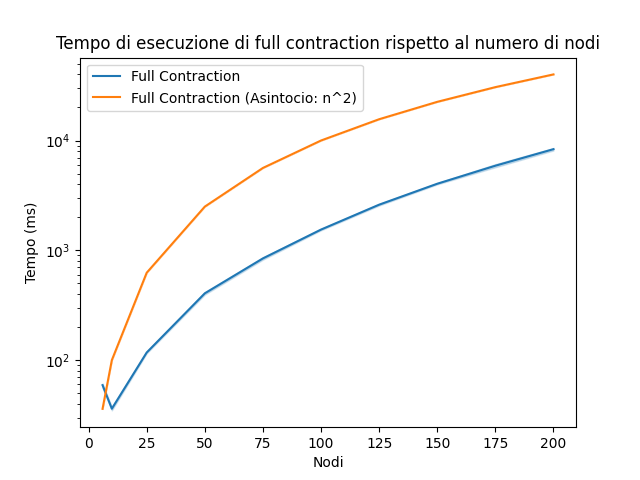
\includegraphics[width=0.9\textwidth]{./images/Tempo_di_esecuzione_di_full_contraction_rispetto_al_numero_di_nodi.png}

    \caption{Confronto tra il tempo di esecuzione di \codeinline{full\_contraction} e la sua complessità asintotica rispetto al numero di nodi. Grafico in scala logaritmica.}
    \label{fig:karger-full-contraction-chart}
\end{figure}

\subsection{Domanda \#2}
\label{sec:question-2}

\begin{displayquote}
Misurate i tempi di calcolo dell'algoritmo di Karger sui grafi del
dataset, usando un numero di ripetizioni che garantisca una
probabilità minore o uguale a $\frac{1}{n}$ di sbagliare. Mostrate i
risultati con un grafico che mostri la variazione dei tempi di calcolo
al variare del numero di vertici nel grafo. Confrontate i tempi
misurati con la complessità asintotica dell'algoritmo. \\

\noindent Nelle istanze più grandi, il tempo di calcolo necessario a
completare tutte le iterazioni potrebbe risultare eccessivo. In questo
caso utilizzate un timeout oppure abbassate il numero di ripetizioni
per ottenere tempi di esecuzione ragionevoli.
\end{displayquote}

\noindent Per permettere all'algoritmo di karger un probabilità di
fallimento pari a $\frac{1}{n}$ è necessario settare d = 1 e di
conseguenza ricavare k con la formula vista nella sezione
\ref{sub:karger-success-probability} e quindi:
$$ k = 1 * \frac{n^2}{2} * ln(n)$$

\noindent Il grafico \ref{fig:karger-runtime-chart} mostra il tempo di
calcolo dell'algoritmo di Karger e lo confronta con il tempo
asintotico rispetto al numero di nodi.

\begin{figure}[H]
    \centering

    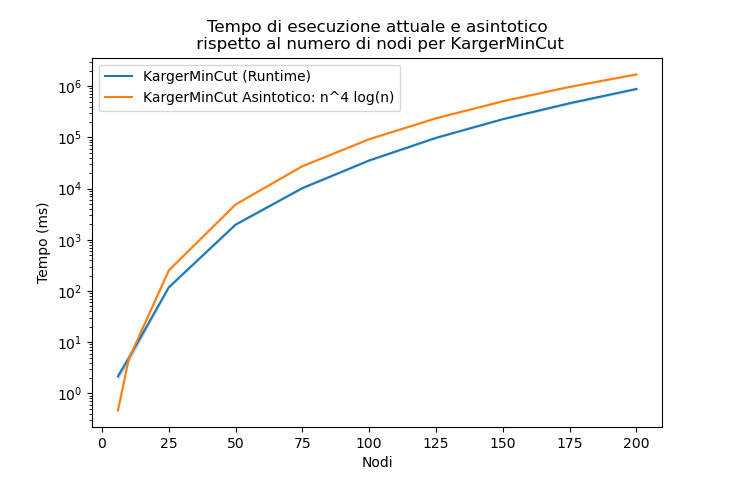
\includegraphics[width=0.9\textwidth]{./images/Tempo_di_esecuzione_attuale_e_asintotico__rispetto_al_numero_di_nodi_per_KargerMinCut.png}

    \caption{Tempo di esecuzione attuale e asintotico per KargerMinCut rispetto al numero di nodi. Grafico in scala logaritmica.}
    \label{fig:karger-runtime-chart}
\end{figure}

\subsection{Domanda \#3}
\label{sec:question-3}

\begin{displayquote}
Misurate il \textit{discovery time} dell'algoritmo di Karger sui grafi
del dataset. Il discovery time è il momento (in secondi) in cui
l'algoritmo trova per la prima volta il taglio di costo mimimo.
Confrontate il discovery time con il tempo di esecuzione complessivo
per ognuno dei grafi nel dataset.
\end{displayquote}

\noindent Il grafico \ref{fig:karger-discovery-vs-program-time-chart}
mostra un confronto per il \emph{runtime}, ovvero il tempo totale di
esecuzione dell'algoritmo e \emph{discovery time}, ovvero il tempo in
cui l'algoritmo trova il taglio di costo minimo per la prima volta.
Le tabelle \ref{table:karger-running-time} e
\ref{table:kargertimeout-running-time} mostrano il dettaglio dei
dati. \\

\noindent È possibile notare che per la curva di \emph{discovery time}
i risultati hanno molta varianza, ma in linea generale essa segue in
modo asintotico quella del \emph{runtime}.\\

\noindent Ovviamente, come ci si può aspettare, la curva
\emph{discovery time} è considerevolmente più bassa rispetto all'altra
in quanto, data la scelta randomica, ``la volta fortunata'' potrebbe
capitare anche prima della fine dell'algorimto, e anzi, spesso è così.

\begin{figure}[H]
    \centering

    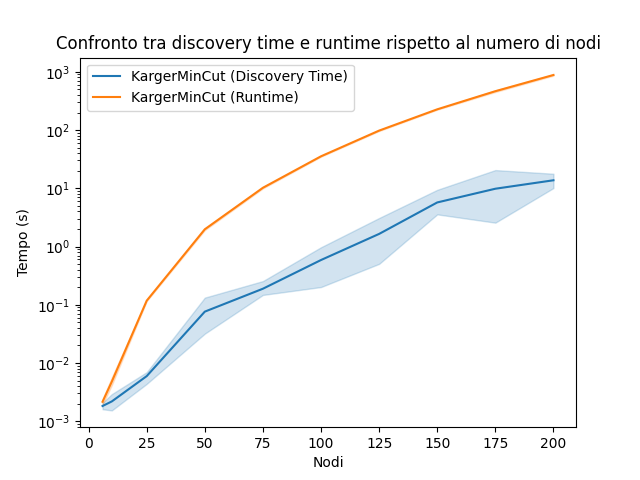
\includegraphics[width=0.9\textwidth]{./images/Confronto_tra_discovery_time_e_runtime_rispetto_al_numero_di_nodi.png}

    \caption{Confronto tra il tempo di esecuzione per \emph{discovery time} e \emph{runtime} rispetto al numero di nodi. Grafico in scala logaritmica.}
    \label{fig:karger-discovery-vs-program-time-chart}
\end{figure}

Il grafico \ref{fig:karger-discovery-vs-estimated-k-chart} invece
illustra una comparativa tra il numero di iterazioni tramite le quali
si trova il min cut e il numero di iterazioni $k$ stimato.

\begin{figure}[!ht]
    \centering

    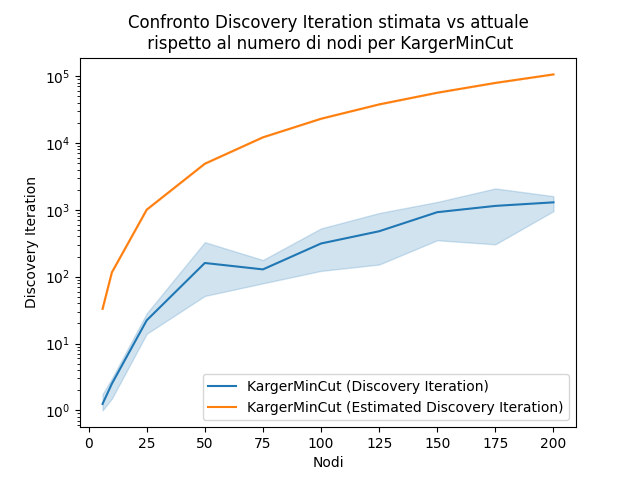
\includegraphics[width=0.9\textwidth]{./images/Confronto_Discovery_Iteration_stimata_vs_attuale__rispetto_al_numero_di_nodi_per_KargerMinCut.png}

    \caption{Confronto discovery iteration stimata vs ottenuta rispetto al numero di nodi per KargerMinCut. Grafico in scala logaritmica.}
    \label{fig:karger-discovery-vs-estimated-k-chart}
\end{figure}

\subsection{Domanda \#4}
\label{sec:question-4}

\begin{displayquote}
Per ognuno dei grafi del dataset, riportate il risultato risultato
ottenuto dalla vostra implementazione, la soluzione attesa e l'errore
relativo calcolato come:

\begin{equation*}
    \frac{SoluzioneTrovata - SoluzioneAttesa}{SoluzioneAttesa}
\end{equation*}

\end{displayquote}

\noindent La nostra implementazione e la scelta del numero di
contrazioni da eseguire non introduce nessun tipo di errore per
l'algoritmo di Karger, quindi un grafico sarebbe poco informatico.\\

\noindent Si ritiene utile invece mostrare le differenza tra
Karger e Karger con Timeout (di seguito KargerMinCutTimeout). Il secondo
differisce dal primo solo perché ad un certo punto l'esecuzione viene
interrotta se l'algoritmo non è ancora terminato.\\

\noindent Dal grafico \ref{fig:karger-vs-kargertout-error-chart} e dal
dettaglio riportato nelle tabelle \ref{table:karger-approx-error} e
\ref{table:kargertimeout-approx-error} è possibile vedere che entrambi
hanno bassissimo errore relativo sull'output, ma Karger impega un
tempo considerevolmente maggiore per risolvere il problema, mentre
KargerMinCutTimeout riesce con successo ad ottenere zero errore anche
prima dello scadere del timeout. Ciò implica che con
KargerMinCutTimeout potrebbe essere utilizzato per avere una soluzione
approssimata entro un tempo accettabile. Quanto descritto è mostrato
nel grafico \ref{fig:karger-vs-kargertout-runtime-chart}.

\begin{figure}[H]
    \centering

    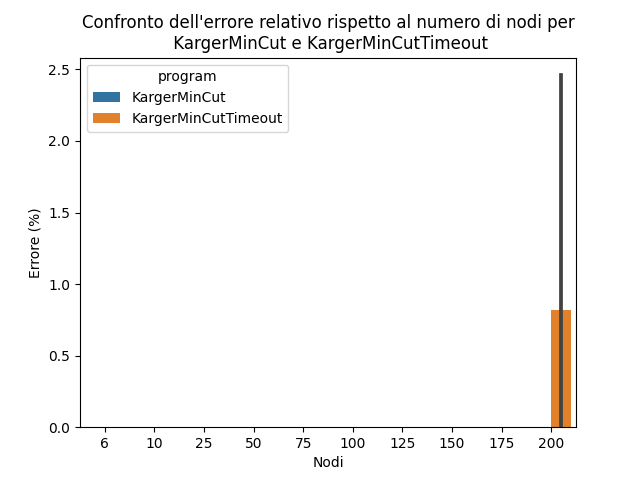
\includegraphics[width=0.9\textwidth]{./images/Confronto_dell'errore_relativo_rispetto_al_numero_di_nodi_per__KargerMinCut_e_KargerMinCutTimeout.png}

    \caption{Confronto dell'errore relativo rispetto al numero di nodi per Karger e Karger con Timeout.}
    \label{fig:karger-vs-kargertout-error-chart}
\end{figure}

\begin{figure}[H]
    \centering

    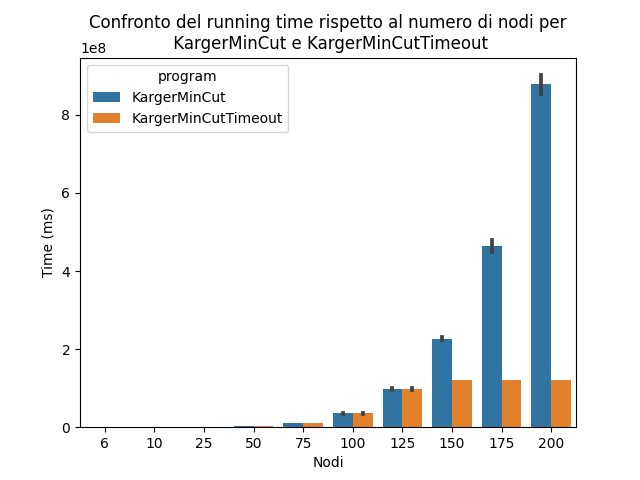
\includegraphics[width=0.9\textwidth]{./images/Confronto_del_running_time_rispetto_al_numero_di_nodi_per__KargerMinCut_e_KargerMinCutTimeout.png}

    \caption{Confronto del running time rispetto al numero di nodi per Karger e Karger con Timeout.}
    \label{fig:karger-vs-kargertout-runtime-chart}
\end{figure}
